\documentclass{article}
\usepackage{graphicx}
\usepackage{fullpage}

\author{Arthur Lui}
\title{624 Midterm 1}

\begin{document}
\maketitle

\section{Harmonic Mean}
  The executable R script, ``harmonic'', computes the 
  harmonic mean of any number of values passed as command 
  line arguments. Below is the content of ``harmonic''.

  \begin{verbatim}
    #!/usr/bin/env Rscript

    x <- as.numeric(commandArgs(T))

    n <- length(x)
    harmonicMean <-  n / sum(1/x)

    harmonicMean
  \end{verbatim}

\section{Day Of Birth}
  The R file, ``birthday.R'', contains the code for this problem.
  \subsection{Compute the $\chi^2$ test statistic}
  The $\chi^2$ statistic for this data is 12.625.
  \subsection{Compute the p-value based on the asymptotic distribution}
  The p-value based on the asymptotic distribution is 0.04939291.
  \subsection{Compute a finite-sample p-value based on Monte Carlo simulation}
  Monte Carlo p-value (.95 Confidence Interval): 0.04888 (0.04699007, 0.05076993)
  \subsection{Conclusion regarding the null hypothesis}
  As the Monte Carlo p-value (.04888) is less than 0.05, 
  we reject the null hypothesis that local births are 
  equally likely on all days of the week at the .05 
  significance level; and we conclude that local births 
  are not equally likely on all days of the week. 
  \subsection{Advantages and Disadvantages of the Monte Carlo approach}
  The Monte Carlo approach can be taken when there is 
  no convenient or closed form solution to computing 
  a test statistic. The data obtained from Monte 
  Carlo simulations can be easily used to create 
  graphs and infer distributions conveniently.

  However, the Monte Carlo approach takes simulation
  time and computing resources. So it may not be the 
  best choice when a closed form solution is known.
  \subsection{What are the power of the asymptotic and finite sample testing procedures?}
  Asymptotic Power (Confidence Interval): 0.4957000 (0.4859005, 0.5054995)\\
  Finite Sample Testing Power (Confidence Interval): 0.4957000 (0.4859005, 0.5054995)

  \subsection{The Sampling Distribution of The Test Statistic}
  \begin{center}
    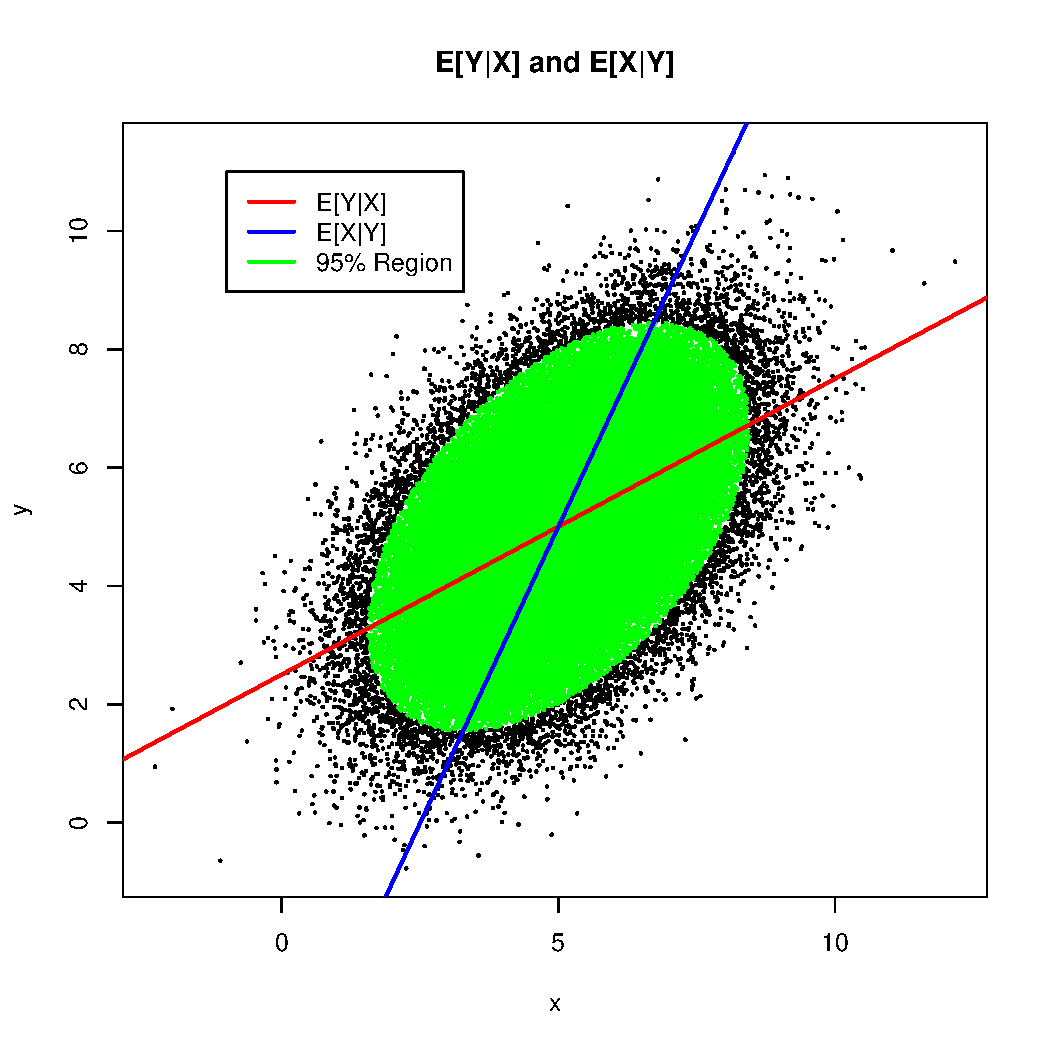
\includegraphics[scale=.8]{plot.pdf}
  \end{center}

\end{document}
